\documentclass[12pt]{article}
\usepackage{latexsym}
\usepackage{url}
\usepackage{hyperref}
\hypersetup{colorlinks=true}
\usepackage{enumitem,amssymb}
\newlist{todolist}{itemize}{4}
\setlist[todolist]{label=$\square$}
\usepackage{clrscode3e}
\usepackage{tikz}
\usepackage{pgfplots}
\usepackage{colortbl}
\usepackage{hyperref}
\usetikzlibrary{calc, shapes, arrows}
\pgfplotsset{compat=1.16}
\begin{document}
\begin{titlepage}
\begin{center}
\huge{\bfseries Chromatic Number}\\
[2 mm]
\line(1,0){300}\\
[2 cm]

\large Iova Daniel-Alexandru\\
[0.3 cm]
\large 1\textsuperscript{st} year, CEN 1.2 B\\
[0.3 cm]
\large Academic Year 2019 - 2020\\
[0.3 cm]
\date{\today}
\end{center}
\end{titlepage}

%===================================================== REQUIREMENT ====================================================
\section{Requirement:}
\textit{Chromatic Number}. Let G be an undirected graph and \textit{k} a natural number greater than zero. We define a \textit{k}-coloring of G an assignment of a color to each node of the graph such that any two adjacent nodes are colored differently. The Chromatic number of G, denoted by $\chi$(G) or $\gamma$(G), is the smallest \textit{k} for which G admits a \textit{k}-coloring. I am tasked with implementing two different algorithms that calculate the chromatic number of a given undirected graph.
\pagebreak
%================================================== PROPOSED ALGORITHMS =================================================
\section{Proposed algorithms:}
%==================================================== 1ST ALGORITHM ====================================================
\subsection{Welsh-Powell-Based Chromatic Number Algorithm}
\begin{codebox}
\Procname{$\proc{Welsh-Powell-Chromatic-Number}(G, N)$}
\li \Comment G is the adjacency matrix of the array, N is the number of nodes
\li $\id{col} \gets 0$
\li $\id{k} \gets 0$
\li \Comment Initialize the array A with the initial nodes and the result array with $-1$.
\li \For $i \gets 0$ \To $N-1$ {\bf do}
\li \Do $A[i] \gets i$
\li $result[i] \gets -1$ \End
\li $\rhd$ Sort the sequence $A[0 \twodots n-1]$ in decreasing order of node degree.
\li \For $i \gets 0$ \To $N-1$ {\bf do}
\li \Do \If $result[A[i]] \isequal -1$ {\bf then}
\li \Do $\id{ok} \gets 0$
\li \For $j \gets 0$ \To $N-1$ {\bf do}
\li \Do \If $G[A[i]][A[j]] \isequal 0$ and $result[A[j]] \isequal -1$ {\bf then}
\li \Do \If $A[j]$ not adjacent to nodes of current color {\bf then}
\li \Do $result[A[j]] \gets \id{col}$
\li $\id{ok} \gets 1$ \End \End \End
\li \If $\id{ok} \isequal 1$ {\bf then}
\li \Do $\id{col} \gets \id{col}+1$ \End \End \End
\li \Comment Calculate the chromatic number as the maximum of the result array + 1
\li \For $i \gets 0$ \To $N-1$ {\bf do}
\li \Do \If $result[i] > \id{k}$ {\bf then}
\li \Do $\id{k} \gets result[i]$ \End \End
\li $\id{k} \gets \id{k} + 1$
\li Return $\id{k}$
\End 
\end{codebox}
\quad
The Welsh and Powell algorithm introduced an upper bound to the chromatic number of a graph. It is a heuristic greedy-based algorithm in which the nodes are sorted by their degree in decreasing order \cite{welsh-powell}. This provides a somewhat more optimal ordering than just randomizing the order of the nodes or just considering the order 0 to n-1 and hoping we get an optimal result. Because this is still a greedy algorithm, the result we are going to obtain is not always the optimal one, but we can expect a suboptimal one. \\ \quad \\
The algorithm consists of the next steps:
\begin{enumerate}
\item Generate array with nodes sorted by degree in decreasing order.
\item Color the first node in the array with the color 0.
\item Continue down the array and color, with the same color, all the nodes not connected to nodes of the same color.
\item Increment the color counter.
\item Repeat the two previous steps on all uncolored nodes until all the nodes are colored
\item The chromatic number will be the maximum element of the coloring array plus 1 (because we started with color 0).
\end{enumerate} \quad \\
\indent The {\bf computational complexity} is {\bf $\mathcal{O}$(N\textsuperscript{2}) }, because we first have $\mathcal{O}$(N) for initializing the A array and result array, $\mathcal{O}$(NlogN) from sorting the array A, $\mathcal{O}$(N\textsuperscript{2}) for when we iterate through the A array and assign colors to the result array and $\mathcal{O}$(N) for when we calculate the maximum of the result array. \quad \\
\indent The {\bf memory requirement} is {\bf $\mathcal{O}$(N\textsuperscript{2})}, because we have $\mathcal{O}$(N\textsuperscript{2}) for storing the input in the adjacency matrix G, $\mathcal{O}$(N) for storing the result array and $\mathcal{O}$(1) for storing the chromatic number. \\ \\ Example: For the following example, the order of vertices after ordering by maximum degree is [1, 4, 0, 2, 3, 5]. The resulting chromatic number is 3 (subscript numbers represent the order of coloring for each color).  \\

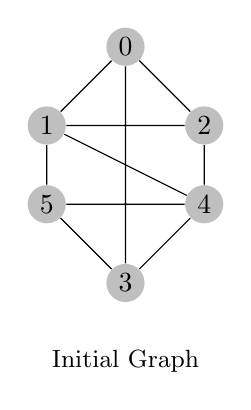
\begin{tikzpicture}
\tikzstyle{vertex}=[circle,fill=black!25,minimum size=12pt,inner sep=2pt]
\node[vertex] (G_0) at (0,0) {0};
\node[vertex] (G_1) at (-1,-1) {1};
\node[vertex] (G_2) at (1,-1)  {2};
\node[vertex] (G_3) at (0, -3) {3};
\node[vertex] (G_4) at (1, -2) {4};
\node[vertex] (G_5) at (-1, -2) {5};
\node at (0,-4) {\small Initial Graph};
\draw (G_0) -- (G_1) -- (G_0) -- (G_2) -- (G_0) -- (G_3) -- (G_0) -- (G_1) -- (G_2) -- (G_4) -- (G_3) -- (G_5) -- (G_1) -- (G_4) -- 
(G_5) -- cycle;
\end{tikzpicture} \indent
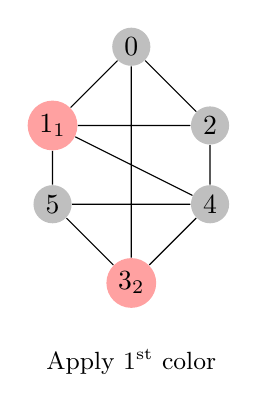
\begin{tikzpicture}
\tikzstyle{vertex}=[circle,fill=black!25,minimum size=12pt,inner sep=2pt]
\tikzstyle{red}=[circle,fill=red!37,minimum size=12pt,inner sep=2pt]
\node[vertex] (G_0) at (0,0) {0};
\node[red] (G_1) at (-1,-1)   {1\textsubscript{1}};
\node[vertex] (G_2) at (1,-1)  {2};
\node[red] (G_3) at (0, -3) {3\textsubscript{2}};
\node[vertex] (G_4) at (1, -2) {4};
\node[vertex] (G_5) at (-1, -2) {5};
\node at (0,-4) { \small Apply 1\textsuperscript{st} color};
\draw (G_0) -- (G_1) -- (G_0) -- (G_2) -- (G_0) -- (G_3) -- (G_0) -- (G_1) -- (G_2) -- (G_4) -- (G_3) -- (G_5) -- (G_1) -- (G_4) -- (G_5) -- cycle;
\end{tikzpicture} \indent
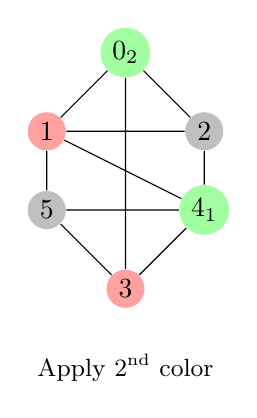
\begin{tikzpicture}
\tikzstyle{vertex}=[circle,fill=black!25,minimum size=12pt,inner sep=2pt]
\tikzstyle{red}=[circle,fill=red!37,minimum size=12pt,inner sep=2pt]
\tikzstyle{green}=[circle,fill=green!37,minimum size=12pt,inner sep=2pt]
\node[green] (G_0) at (0,0) {0\textsubscript{2}};
\node[red] (G_1) at (-1,-1)   {1};
\node[vertex] (G_2) at (1,-1)  {2};
\node[red] (G_3) at (0, -3) {3};
\node[green] (G_4) at (1, -2) {4\textsubscript{1}};
\node[vertex] (G_5) at (-1, -2) {5};
\node at (0,-4) { \small Apply 2\textsuperscript{nd} color};
\draw (G_0) -- (G_1) -- (G_0) -- (G_2) -- (G_0) -- (G_3) -- (G_0) -- (G_1) -- (G_2) -- (G_4) -- (G_3) -- (G_5) -- (G_1) -- (G_4) -- (G_5) -- cycle;
\end{tikzpicture} \indent
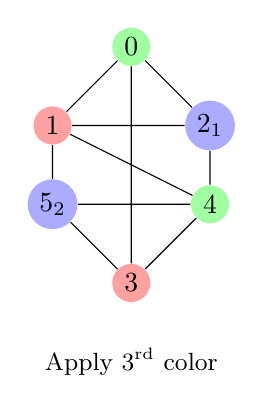
\begin{tikzpicture}
\tikzstyle{red}=[circle,fill=red!37,minimum size=12pt,inner sep=2pt]
\tikzstyle{green}=[circle,fill=green!37,minimum size=12pt,inner sep=2pt]
\tikzstyle{blue}=[circle,fill=blue!33,minimum size=12pt,inner sep=2pt]
\node[green] (G_0) at (0,0) {0};
\node[red] (G_1) at (-1,-1)   {1};
\node[blue] (G_2) at (1,-1)  {2\textsubscript{1}};
\node[red] (G_3) at (0, -3) {3};
\node[green] (G_4) at (1, -2) {4};
\node[blue] (G_5) at (-1, -2) {5\textsubscript{2}};
\node at (0,-4) { \small Apply 3\textsuperscript{rd} color};
\draw (G_0) -- (G_1) -- (G_0) -- (G_2) -- (G_0) -- (G_3) -- (G_0) -- (G_1) -- (G_2) -- (G_4) -- (G_3) -- (G_5) -- (G_1) -- (G_4) -- (G_5) -- cycle;
\end{tikzpicture} \indent
%==================================================== 2ND ALGORITHM ====================================================
\subsection{Modified M-Coloring Algorithm}
\begin{codebox}
\Procname{$\proc{M-Coloring-Chromatic-Number}(G, N)$}
\li \Comment G is the adjacency matrix of the array, N is the number of nodes.
\li \Comment G is used when testing if it safe to color the nodes for the color config.
\li $\id{K} \gets 1$
\li $\rhd$ Generate color configuration array with $\id{K}$ colors.
\li \If color configuration incomplete {\bf then}
\li \Do \While color configuration incomplete {\bf do}
\li \Do $\id{K}  \gets \id{K} + 1$
\li $\rhd$ Generate color configuration array with $\id{K}$ colors. \End \End
\li Return $\id{K}$
\End 
\end{codebox} \quad \\
\indent The m-Coloring problem requires that we test if a given undirected graph is colored with a given m. It uses backtracking to generate a color configuration for the given m, and if it is incomplete, returns false, otherwise returns true \cite{m-col}. \\ 
\indent I have modified this algorithm by making m a variable that starts from 1 and is incremented until the generated color configuration is complete. \\
\indent The color configuration is generated by coloring each vertex, starting from vertex 0, such that, before assigning a color, we check if the node is adjacent to any nodes of the same color. If it is safe to color the node, assign it a color and add it to the current color configuration. If no colors are assigned, backtrack and return false. \\
\indent The {\bf computational complexity} of the algorithm is {\bf $\mathcal{O}$($\sum_{i=1}^{K} i^N$) } because there are K\textsuperscript{N} possible combinations, with K starting from 1 and incrementing itself until it reaches the chromatic number.\\
\indent The {\bf memory requirement} of the algorithm is {\bf $\mathcal{O}$(N\textsuperscript{2})}, because we have $\mathcal{O}$(N\textsuperscript{2}) for storing the input in the adjacency matrix G, $\mathcal{O}$(N) for storing the color configuration array and $\mathcal{O}$(1) for storing the resulting chromatic number. \\ \\ Example: For the following example, the chromatic number (denoted by K) starts from 1 and increments itself until a complete combination is found. The order in which the nodes are colored is irrelevant, so the example shows one of the possible combinations (color 0 - red, color 1 - green, color 2 - blue). \\

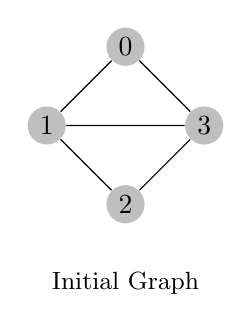
\begin{tikzpicture}
\tikzstyle{vertex}=[circle,fill=black!25,minimum size=12pt,inner sep=2pt]
\node[vertex] (G_0) at (0,0) {0};
\node[vertex] (G_1) at (-1,-1)   {1};
\node[vertex] (G_2) at (0, -2) {2};
\node[vertex] (G_3) at (1,-1)  {3};
\node at (0,-3) {\small Initial Graph};
\draw (G_0) -- (G_1) -- (G_2) -- (G_3) -- (G_1) -- (G_0) -- (G_3) -- cycle;
\end{tikzpicture} \indent
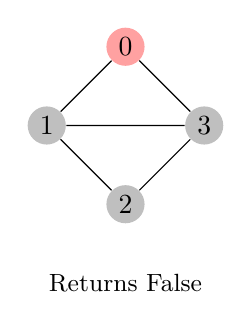
\begin{tikzpicture}
\tikzstyle{vertex}=[circle,fill=black!25,minimum size=12pt,inner sep=2pt]
\tikzstyle{red}=[circle,fill=red!37,minimum size=12pt,inner sep=2pt]
\node[red] (G_0) at (0,0) {0};
\node[vertex] (G_1) at (-1,-1)   {1};
\node[vertex] (G_2) at (0, -2) {2};
\node[vertex] (G_3) at (1,-1)  {3};
\node at (0,-3) {\small Returns False};
\draw (G_0) -- (G_1) -- (G_2) -- (G_3) -- (G_1) -- (G_0) -- (G_3) -- cycle;
\end{tikzpicture} \indent
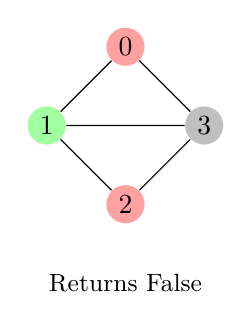
\begin{tikzpicture}
\tikzstyle{vertex}=[circle,fill=black!25,minimum size=12pt,inner sep=2pt]
\tikzstyle{red}=[circle,fill=red!37,minimum size=12pt,inner sep=2pt]
\tikzstyle{green}=[circle,fill=green!37,minimum size=12pt,inner sep=2pt]
\node[red] (G_0) at (0,0) {0};
\node[green] (G_1) at (-1,-1)   {1};
\node[red] (G_2) at (0, -2) {2};
\node[vertex] (G_3) at (1,-1)  {3};
\node at (0,-3) {\small Returns False};
\draw (G_0) -- (G_1) -- (G_2) -- (G_3) -- (G_1) -- (G_0) -- (G_3) -- cycle;
\end{tikzpicture} \indent
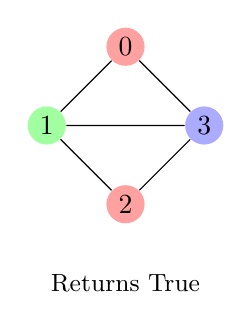
\begin{tikzpicture}
\tikzstyle{red}=[circle,fill=red!37,minimum size=12pt,inner sep=2pt]
\tikzstyle{green}=[circle,fill=green!37,minimum size=12pt,inner sep=2pt]
\tikzstyle{blue}=[circle,fill=blue!33,minimum size=12pt,inner sep=2pt]
\node[red] (G_0) at (0,0) {0};
\node[green] (G_1) at (-1,-1)   {1};
\node[red] (G_2) at (0, -2) {2};
\node[blue] (G_3) at (1,-1)  {3};
\node at (0,-3) {\small Returns True};
\draw (G_0) -- (G_1) -- (G_2) -- (G_3) -- (G_1) -- (G_0) -- (G_3) -- cycle;
\end{tikzpicture} \indent

%=================================================== EXPERIMENTAL DATA ==================================================
\section{Experimental data:} \quad \\
\indent The non-trivial data is created using an algorithm which firstly generates a random number of nodes N. Then, for a random number of lines, generates two integers in range [0..N-1] and adds the pair to an array of pairs. The array is then cleaned up by removing inverted duplicates (i.e. we have "a b" and "b a" in the array so we remove either one of them) and pairs with same value for  both members (i.e "a a", "b b"). In the end we print N, followed by the lines of pairs. The data is output to a file which will become one of the input files for the two algorithms. \quad \\
\indent Because the data is to be run on both algorithms and one of them is a backtracking algorithm, the input cannot consist of big values (the number of distinct edges cannot be greater than $\approx$70 edges for the Python implementation and $\approx$120 edges for the C implementation). On the other hand, the greedy algorithm can run inputs of more than $\approx$800 edges while still outputting a sub-optimal or even optimal result. The downside to running big inputs on the greedy algorithm is that, because this problem is only correctly solved by a brute-force/backtracking approach \cite{brittanica}, we will never be able to test if the result is correct or not in a reasonable amount of time (or at all). \\
\indent The generated data is significant for testing because it shows the difference in performance and speed between the two algorithms, but also because it shows the difference in speed between the Python and C implementations. \pagebreak

%============================================ EXPERIMENTAL APPLICATION DEVELOPMENT ===========================================
\section{Experimental application development:}

Following are the high-level structures of both algorithms in their C implementations along with descriptions of their modules and procedures.
%==================================================== 1ST ALGORITHM ====================================================
\subsection{1\textsuperscript{st} Algorithm:}  \quad \\
\begin{center}
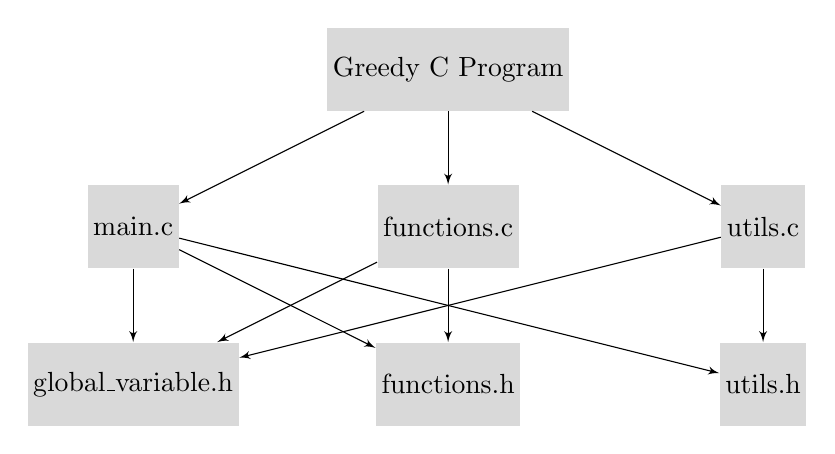
\begin{tikzpicture}
\tikzstyle{line} = [draw, -latex']
\tikzstyle{vertex}=[rectangle,fill=black!15,minimum size=30pt,inner sep=2pt]
\node[vertex] (G_0) at (0,0) {Greedy C Program};
\node[vertex] (G_1) at (-4,-2) {main.c};
\node[vertex] (G_2) at (0,-2) {functions.c};
\node[vertex] (G_3) at (4,-2) {utils.c};
\node[vertex] (G_4) at (-4,-4) {global\_variable.h};
\node[vertex] (G_5) at (0,-4) {functions.h};
\node[vertex] (G_6) at (4,-4) {utils.h};
\path [line] (G_0) -- (G_1);
\path [line] (G_0) -- (G_2);
\path [line] (G_0) -- (G_3);
\path [line] (G_1) -- (G_4);
\path [line] (G_1) -- (G_5);
\path [line] (G_1) -- (G_6);
\path [line] (G_2) -- (G_4);
\path [line] (G_3) -- (G_4);
\path [line] (G_2) -- (G_5);
\path [line] (G_3) -- (G_6);
\end{tikzpicture}
\end{center} \quad \\
Modules and their respective procedures:
\begin{itemize}
\item \textit{main.c}
\begin{itemize}
\item Main program module
\item Procedures: \begin{itemize}\item \textbf{int main()} - main function of the program\end{itemize}
\end{itemize}
\item \textit{generate\_array.c}
\begin{itemize}
\setlength\itemsep{1em}
\item Module with procedures that generate the array with sorted nodes
\item Procedures are declared in the header \textit{generate\_array.h}
\item Procedures:
\begin{itemize}
\setlength\itemsep{1em}
\item \textbf{int degree\_of\_node(int node)} - returns degree of given node
\item \textbf{int cmp(const void *a, const void*b)} - comparator function for qsort which uses previous function for comparison
\item \textbf{void generate\_list\_by\_degree(int array[], int no\_nodes)} - generates the array using the previous functions and C's qsort
\end{itemize}
\end{itemize}
\item \textit{utils.c}
\begin{itemize}
\item Multi-purpose module which includes functions that range from input-output handling to assigning colors to the result array
\item Procedures are declared in the header \textit{utils.h}
\item Procedures:
\begin{itemize}
\setlength\itemsep{1em}
\item \textbf{int check\_connected\_same\_color(int node, int color)} - checks if any node adjacent to the given node has the same color as given color
\item \textbf{void assign\_color(int node, int vertex\_order[])} - procedure to assign colors to the result array
\item \textbf{void read\_data(const char* file)} - reads data from given file and assigns it to the global variables
\item \textbf{void print\_result(const char* file)} - computes and prints the chromatic number to given file
\end{itemize}
\end{itemize}
\end{itemize} \pagebreak
%==================================================== 2ND ALGORITHM ====================================================
\subsection{2\textsuperscript{nd} Algorithm:} \quad \\
\begin{center}
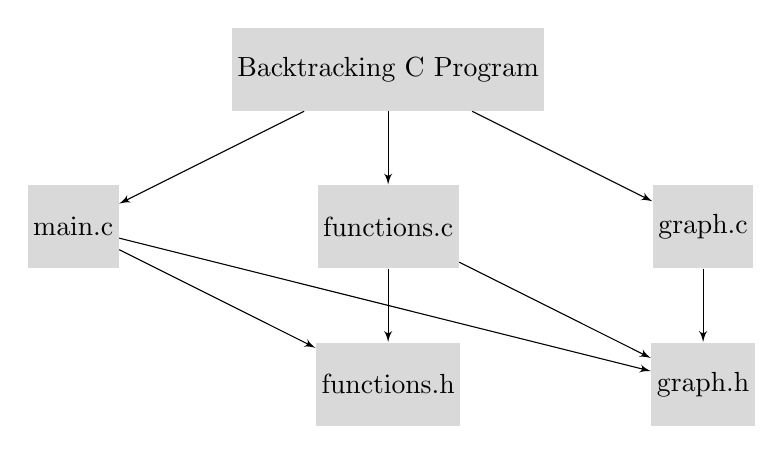
\begin{tikzpicture}
\tikzstyle{line} = [draw, -latex']
\tikzstyle{vertex}=[rectangle,fill=black!15,minimum size=30pt,inner sep=2pt]
\node[vertex] (G_0) at (0,0) {Backtracking C Program};
\node[vertex] (G_1) at (-4,-2) {main.c};
\node[vertex] (G_2) at (0,-2) {functions.c};
\node[vertex] (G_3) at (4,-2) {graph.c};
\node[vertex] (G_5) at (0,-4) {functions.h};
\node[vertex] (G_6) at (4,-4) {graph.h};
\path [line] (G_0) -- (G_1);
\path [line] (G_0) -- (G_2);
\path [line] (G_0) -- (G_3);
\path [line] (G_1) -- (G_5);
\path [line] (G_1) -- (G_6);
\path [line] (G_2) -- (G_5);
\path [line] (G_2) -- (G_6);
\path [line] (G_3) -- (G_6);

\end{tikzpicture}
\end{center} \quad \\
Modules and their respective procedures:
\begin{itemize}
\item \textit{main.c}
\begin{itemize}
\item Main program module
\item Procedures: \begin{itemize}\item \textbf{int main()} - main function of the program in which the final coloring function is called until a valid combination is found; prints the computed chromatic number to an output file\end{itemize}
\end{itemize}
\item \textit{functions.c}
\begin{itemize}
\item Module responsible for I/O functions
\item Procedure is declared in the header \textit{functions.h}
\item Procedure:
\begin{itemize}
\item \textbf{void read\_data(struct Graph* g, const char* file)} - reads input from file and assigns it to a "Graph" structure g
\end{itemize}
\end{itemize}
\item \textit{graph.c}
\begin{itemize}
\item Module solely involved with graph related procedures
\item Procedures and structure "Graph" are declared in the header \textit{graph.h}
\item Procedures:
\begin{itemize}
\setlength\itemsep{1em}
\item \textbf{int safe\_to\_color(struct Graph g, int vertex, int coloring\_result[], int color)} - checks if given vertex is safe to color (no adjacent node has the same color)
\item \textbf{int graph\_color\_utility\_function(struct Graph g, int chromatic\_number, int coloring\_result[], int vertex)} - recursive utility procedure used to build the coloring\_result array
\item \textbf{int final\_coloring\_function(struct Graph g, int chromatic\_number, int coloring\_result[])} - final coloring function in which the coloring result is built by calling the previous function
\end{itemize}
\end{itemize}
\end{itemize}
The Python implementation of this algorithm uses a class, with everything inside C's "graph.c" being procedures of said class.
\subsection{Common Traits:}
To change what input file is to be run: \\
\indent - For the {\bf C} implementations: \\
\indent \indent - Change the "INPUT\_INDEX" macro inside "main.c". \\
\indent \indent - Build and Run the program. \\
\indent - For the {\bf Python} implementations: \\
\indent \indent - Change the "input\_index" variable inside "main.py". \\
\indent \indent - Save and Run the program. \\ \\
\indent Input data consists of values in range of [1..100] nodes and [0..150] edges. It is of the following format:\\
\textit{\textbf{n}} \\
\textit{\textbf{x\textsubscript{0} y\textsubscript{0}}} \\
\textit{\textbf{x\textsubscript{1} y\textsubscript{1}}} \\
\textit{\textbf{x\textsubscript{2} y\textsubscript{2}}} \\
\textbf{...} \\
where \textit{\textbf{n}} is the number of nodes and the number of edges (\textit{\textbf{x\textsubscript{i} y\textsubscript{i}}}) is random.
Output data is an integer representing the computed chromatic number.
%================================================= RESULTS & CONCLUSIONS =================================================
\section{Results and Conclusions:}  \quad \\
\indent Both algorithms output a single integer: the chromatic number of the given graph. Running the algorithms on 10 input files, we can see in the table below that the greedy algorithm has a 60\% success rate, while the backtracking one returns the optimal answer everytime. With that being said, the wrong outputs are still sub-optimal. \\
\indent To test the correctness of their output, I used an online tool called "SageMathCell" \cite{sagemathcell}, which is an online wrapper for the mathematics software system SageMath.  \\ \\
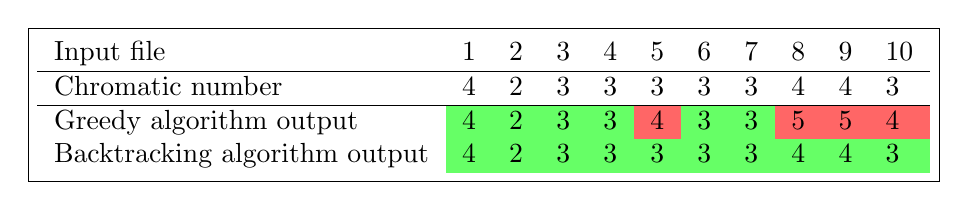
\begin{tikzpicture}
\node[anchor=north,fill=white,draw=black] {\begin{tabular}{l l l l l l l l l l l}
		Input file & 1 & 2 & 3 & 4 & 5 & 6 & 7 & 8 & 9 & 10 \\
		\hline
		Chromatic number & 4 & 2 & 3 & 3 & 3 & 3 & 3 & 4 & 4 & 3 \\
		\hline
		Greedy algorithm output & \cellcolor{green!60}4 & \cellcolor{green!60}2 & \cellcolor{green!60}3 & \cellcolor{green!60}3 & \cellcolor{red!60}4 & \cellcolor{green!60}3 & \cellcolor{green!60}3 & \cellcolor{red!60}5 & \cellcolor{red!60}5 & \cellcolor{red!60}4 \\
		Backtracking algorithm output &\cellcolor{green!60}4 & \cellcolor{green!60}2 & \cellcolor{green!60}3 & \cellcolor{green!60}3 & \cellcolor{green!60}3 & \cellcolor{green!60}3 & \cellcolor{green!60}3 & \cellcolor{green!60}4 & \cellcolor{green!60}4 & \cellcolor{green!60}3    
\end{tabular}};
\end{tikzpicture} \\ \\
\indent Below are graphs of the execution time differences between the C and Python implementations of each algorithm. I chose to split the representation in 2 different graphs because this allows me to better show the difference. If I were to represent all of them on the same graph, the first algorithm's representations would be glued to 0 on the X axis. 
\begin{center}
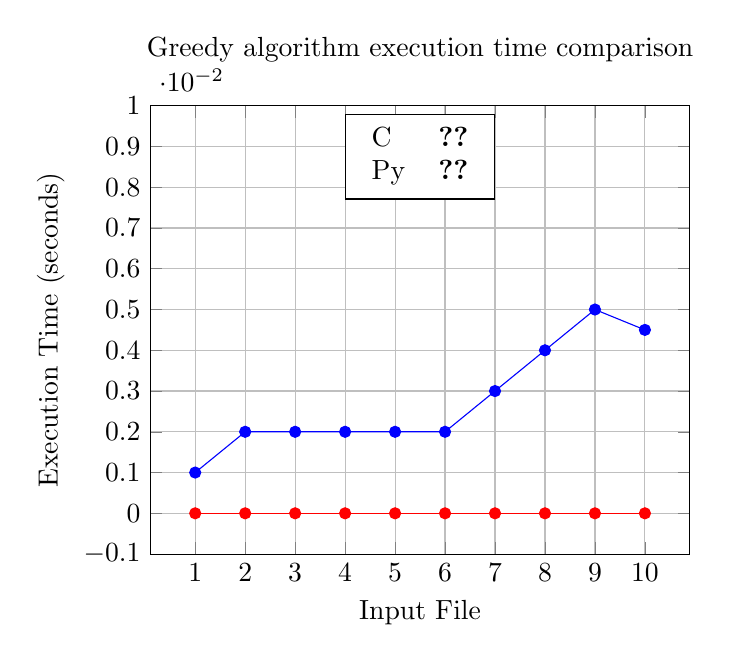
\begin{tikzpicture}
	\begin{axis}[
		title = Greedy algorithm execution time comparison,
		title style={yshift=1.5ex},
		name = plot,
		xtick distance = 1,
		ytick distance = .001,
		ymax = .01,
		grid = both,
		xlabel=Input File,
		ylabel=Execution Time (seconds)]
	\addplot[color=blue, mark=*] coordinates {
		(1,0.001)
		(2,0.002)
		(3,0.002)
		(4,0.002)
		(5,0.002)
		(6,0.002)
		(7,0.003)
		(8,0.004)
		(9,0.005)
		(10,0.0045)
	};\label{Py}
	\addplot[color=red, mark=*] coordinates {
		(1,0)
		(2,0)
		(3,0)
		(4,0)
		(5,0)
		(6,0)
		(7,0)
		(8,0)
		(9,0)
		(10,0)
	};\label{C}
	\end{axis}
	\node[anchor=north,fill=white,draw=black] (legend) at ($(plot.north)-(0 mm, 1 mm)$) {\begin{tabular}{l l}
		C & \ref{C} \\
		Py & \ref{Py}
    \end{tabular} };
\end{tikzpicture} 
\end{center}
\indent For this first graph, we can see a clear difference between the execution times of the Python and C implementations. This is a negligible difference though, with the values being in the range of 0 to 0.005 seconds. \\
\begin{center}
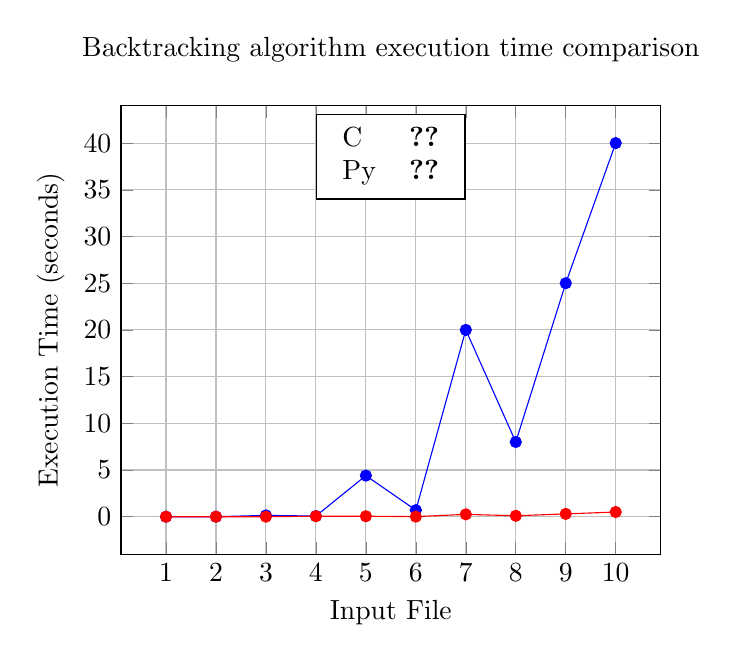
\begin{tikzpicture}
	\begin{axis}[
		title = Backtracking algorithm execution time comparison,
		title style={yshift=1.5ex},
		name = plot,
		xtick distance = 1,
		ytick distance = 5,
		grid = both,
		xlabel=Input File,
		ylabel=Execution Time (seconds)]
	\addplot[color=blue, mark=*] coordinates {
		(1,0.0)
		(2,0.001)
		(3,0.14)
		(4,0.07)
		(5,4.4)
		(6,0.7)
		(7,20)
		(8,8)
		(9,25)
		(10,40)
	};\label{Py2}
	\addplot[color=red, mark=*] coordinates {
		(1,0)
		(2,0)
		(3,0.001)
		(4,0.051)
		(5,0.051)
		(6,0.008)
		(7,0.25)
		(8,0.1)
		(9,0.3)
		(10,0.5)
	};\label{C2}
	\end{axis}
	\node[anchor=north,fill=white,draw=black] (legend) at ($(plot.north)-(0 mm, 1 mm)$) {\begin{tabular}{l l}
		C & \ref{C2} \\
		Py & \ref{Py2}
    \end{tabular} };
\end{tikzpicture}
\end{center}
\indent For this second graph, we can see the massive difference between the execution times. It seems Python is continuing to be the slowest between the two, getting up to 80 times slower than the C implementation. In comparison, Python's slowness starts to show in the first algorithm when the node count is $\approx$10\textsuperscript{5} with more than $\approx$500 edges (getting around 3 times slower than it's C counterpart).\\ \\ \indent The results show the staggering difference between the two algorithms (reaching up to an 8000 times difference between their worst cases). For the first one we trade correctness for speed, while for the second we do the exact opposite. Even though we cannot test inputs of larger size it is still interesting to see how the greedy algorithm starts to give faulty answers or how the backtracking one struggles with time under a regular-sized input. \\ \\
\indent This was an interesting and complicated project to create, with the most difficult part of it being the C implementation. With the lack of classes and the easiness of writing Python code, writing in C felt more like a chore. It did pay off though, with the blazing fast execution times. This cannot be said about the 2\textsuperscript{nd} implementation as much, with one of the future goals of this project being to optimize the backtracking algorithm more so that it can process larger inputs. All in all it was a great learning experience which helped my algorithmic skills grow.
%===================================================== REFERENCES =====================================================
\begin{thebibliography}{9}
\bibitem{welsh-powell}
Aslan Murat, and Baykan Nurdan. 
\textit{A Performance Comparison of Graph Coloring Algorithms}. 
International Journal of Intelligent Systems and Applications in Engineering, 2016.

\bibitem{m-col}
Article on a backtracking m-Colorability algorithm,
\\\url{https://www.includehelp.com/algorithms/graph-coloring-problem-solution-using-backtracking-algorithm.aspx}

\bibitem{brittanica}
Article on NP-Completeness,
\\\url{https://www.britannica.com/science/NP-complete-problem}

\bibitem{sagemathcell}
SageMathCell, web interface to the free open-source mathematics software system SageMath,
\\\url{https://sagecell.sagemath.org}

\end{thebibliography}
\end{document}